\begin{frame}{Постановка задачі}
	\manimate
	Користувачі мають 2 матриці розмірів $N \times N$ та хочуть обрахувати їх добуток у розподіленому середовищі.
	Між користувачами виникає конфлікт, оскільки у них спільний, рівноправний та конкурентний доступ до розподіленого середовища. 
\end{frame}

\begin{frame}{Структура Cloud середовища}
	\manimate
	
	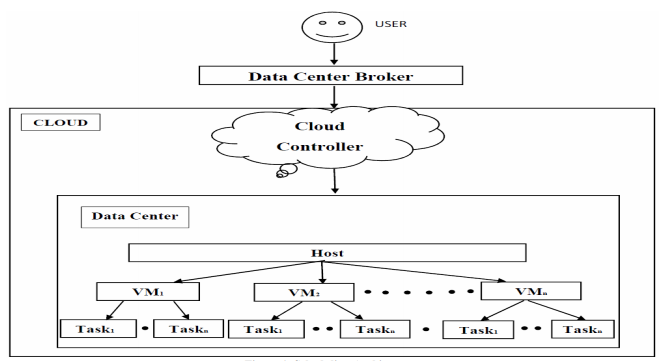
\includegraphics[width=1.0\linewidth]{im/cloud_representation}
\end{frame}

\begin{frame}{Множення матриць блочно}
	\manimate
	Для матриць розмірів $N \times N$ вибирається розмір розрізання $n: n \bigm| N, k = \frac{N}{n}$. Отримуємо $k^2$ задач множення матриць $n \times N$ та $N \times n$.
	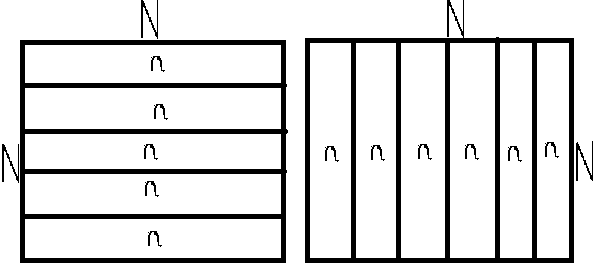
\includegraphics[width=0.8\linewidth]{im/matrixmatrix}
\end{frame}

\begin{frame}{Потокова модель}
	\manimate
	\centering
	\includegraphics[width=0.7\linewidth]{im/fluid_model}
	
	$V$ - загальний об'єм рідини.

	$P = \sum_{i=1}^{m} p_i$ - загальна пропускна здатність посудин.
	
	$x_i = \frac{p_i}{P}$.
	
	$v_i = V * x_i$ - об'єм води для посудини $i$.

\end{frame}

\begin{frame}{Потокова модель}
	\manimate
	\centering
	
	\begin{equation*}
		T_s(x,X(n)) = \max\limits_{i=1,\ldots,m} \bigg\{ d_i \frac{N^3}{p_i} + d_i \frac{N^2 ( 1 + 2*\frac{N}{n} )}{q} + d_i \frac{N^2}{n^2} l \bigg\}
	\end{equation*}
	
	$N$ - розмір матриць

	$n$ - розмір розбиття	
	
	$p_i$ - потужність вузла $i$
	
	$d_i$ - доля обчислень вузла $i$
	
	$q$ - ширина каналу передачі даних $i$
	
	$l$ - час на створення з'єднання

\end{frame}

\begin{frame}{Потокова модель (дискретний варіант)}
	\manimate
	\centering
	$K = \frac{N^2}{n^2}$ - загальна кількість задач однакової складності множення матриць $n*N$ та $N*n$

	$\hat{k_i} = d_i * K$

	$k_i: \sum_{i=1}^{m} |k_i - \hat{k_i}| \Rightarrow min$ - кількість задач, обчислених на вузлі $i$

\end{frame}

\begin{frame}{Пояснення штрафів}
	\manimate
	\centering
	
	У випадку коли матриця $N*N$ не розрізається, то передаються 2 матриці $A,B$ та результат $C=AB$. Тобто передається $3*N*N$ елементів.
	
	При розбитті $n$ формується $K = \frac{N^2}{n^2}$ задач для кожної задачі передається $n*N + N*n + n*n$ елементів. Тобто у загальному це $\frac{N^2*(n*N + N*n + n*n)}{n^2}$.Або $N^2*(2\frac{N}{n}+1)$.
	
	Порівнюючи це з випадком без розрізання маємо: $\frac{2\frac{N}{n}+1}{3}$.
	
\end{frame}

\begin{frame}{Ігрова постановка задачі}
	\manimate
	Гра двох користувачів:
	\begin{itemize}
		\item[1.] Користувачі вибирають розбиття $n_1, n_2$.
		\item[2.] Користувачі розрізають матриці, формують задачі та надсилають їх до хмари.
		\item[3.] Користувачі отримують результати.
	\end{itemize}
	Часом для користувача вважається час отримання усіх результатів надісланих задач.
\end{frame}

\begin{frame}{Ігрова постановка задачі}
	\manimate
	Таким чином отримано біматричну гру з матрицями програшів $(A,B)$.
	
	Стратегіями користувачів є саме їх вибране розбиття. $A^T = B$ оскільки час для гравця 1 у випадку профілю стратегій $(n_1, n_2)$ дорівнює часу гравця 2 з профілем стратегій $(n_2, n_1)$.
	
\end{frame}

\begin{frame}{Ігрова постановка задачі}
\manimate

	Досліджувані планувальники - статичні планувальники типу extr-extr.
	
	min-min - посилає задачу із черги з найменшою складністю на обчислювальний вузол с найменшою потужністю.

\end{frame}